\chapter{Lab 5 - Operational Amplifiers}

%%%%%%%%%%%%%%%%%%%%%%%%%%%%%%%%%%%%%%%%%%%%%%%%%%%%%%%%%%%%%%%%%%%%%%%%%%%%%%%%%%%%%%%%%%%%%%%%%%%%%%%
\section{Objective}
%%%%%%%%%%%%%%%%%%%%%%%%%%%%%%%%%%%%%%%%%%%%%%%%%%%%%%%%%%%%%%%%%%%%%%%%%%%%%%%%%%%%%%%%%%%%%%%%%%%%%%%

The purpose of this lab is to introduce  operational amplifiers through the ideal op amp model, spice op amp model, and practical applications of op amps in common configurations. 

%%%%%%%%%%%%%%%%%%%%%%%%%%%%%%%%%%%%%%%%%%%%%%%%%%%%%%%%%%%%%%%%%%%%%%%%%%%%%%%%%%%%%%%%%%%%%%%%%%%%%%%
\section{Materials}
%%%%%%%%%%%%%%%%%%%%%%%%%%%%%%%%%%%%%%%%%%%%%%%%%%%%%%%%%%%%%%%%%%%%%%%%%%%%%%%%%%%%%%%%%%%%%%%%%%%%%%%

\begin{itemize}
	\item Laptop with LTSpice
	\item Analog Discovery
	\item Breadboard
	\item Wiring kit
	\item Lab parts kit with TLV272
\end{itemize}

%%%%%%%%%%%%%%%%%%%%%%%%%%%%%%%%%%%%%%%%%%%%%%%%%%%%%%%%%%%%%%%%%%%%%%%%%%%%%%%%%%%%%%%%%%%%%%%%%%%%%%%
\section{Introduction}
%%%%%%%%%%%%%%%%%%%%%%%%%%%%%%%%%%%%%%%%%%%%%%%%%%%%%%%%%%%%%%%%%%%%%%%%%%%%%%%%%%%%%%%%%%%%%%%%%%%%%%%

There is a large variety of op amp and specialized amplifiers. For this lab the more recent TLV272 is used, a dual op amp, which contains two op amps, or channels, in a single chip.

%%%%%%%%%%%%%%%%%%%%%%%%%%%%%%%%%%%%%%%%%%%%%%%%%%%%%%%%%%%%%%%%%%%%%%%%%%%%%%%%%%%%%%%%%%%%%%%%%%%%%%
\subsection{The Ideal Op Amp}
%%%%%%%%%%%%%%%%%%%%%%%%%%%%%%%%%%%%%%%%%%%%%%%%%%%%%%%%%%%%%%%%%%%%%%%%%%%%%%%%%%%%%%%%%%%%%%%%%%%%%%

Recall that an ideal op amp will have the following properties. 

\begin{itemize}
	\item Zero input current, often called the input bias current and represented as $\mathrm{I_B}$ or $\mathrm{I_{IB}}$. 
	\item Zero input offset voltage, represented as either $\mathrm{V_{IO}}$ or $\mathrm{V_{OS}}$.
	\item Infinite input resistance, represented as $\mathrm{R_{in}}$ or $\mathrm{r_i}$.  
	\item Zero output resistance, represented as $\mathrm{R_{out}}$ or $\mathrm{r_o}$.
	\item Infinite gain, represented as A or $\alpha$ and often called the open loop gain.
\end{itemize}

\noindent These quantities are represented in \hyperref[fig:IdealAmp]{Figure \ref*{fig:IdealAmp}}.

\begin{figure}[h]
	\centering
		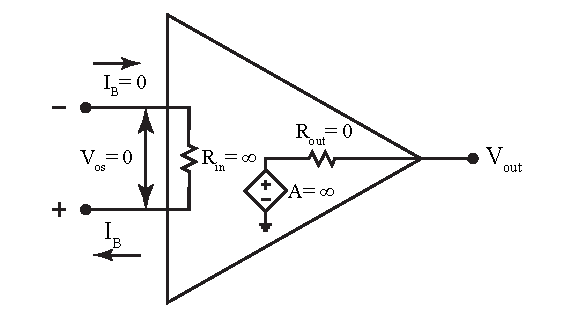
\includegraphics[width=0.5\textwidth]{Lab4idealOpAmp.pdf}
	\caption{Basic op amp model.} \label{fig:IdealAmp}
\end{figure}

However, as should be expected, practical op amp do not have these ideal quantities. For example, the Texas Instrument's TLV272 has finite values for all of the ideal properties. Note that these values vary and depend on productions variation, temperature, and supply voltage.

\begin{itemize}
	\item Finite input bias current, typically 1 pA.
	\item Finite input offset voltage, typically 0.5 mV.
	\item Finite input resistance, typically 1,000 G$\Omega$ differential input resistance.
	\item Finite gain, typically 115 dB (563k)
\end{itemize}

%%%%%%%%%%%%%%%%%%%%%%%%%%%%%%%%%%%%%%%%%%%%%%%%%%%%%%%%%%%%%%%%%%%%%%%%%%%%%%%%%%%%%%%%%%%%%%%%%%%%%%
\subsection{Common Configurations}
%%%%%%%%%%%%%%%%%%%%%%%%%%%%%%%%%%%%%%%%%%%%%%%%%%%%%%%%%%%%%%%%%%%%%%%%%%%%%%%%%%%%%%%%%%%%%%%%%%%%%%

There are a variety of configurations op amps can be used for but there are a few common configurations that form the basis of more complicated op amp circuits. 

\begin{figure} [h]
	\centering
		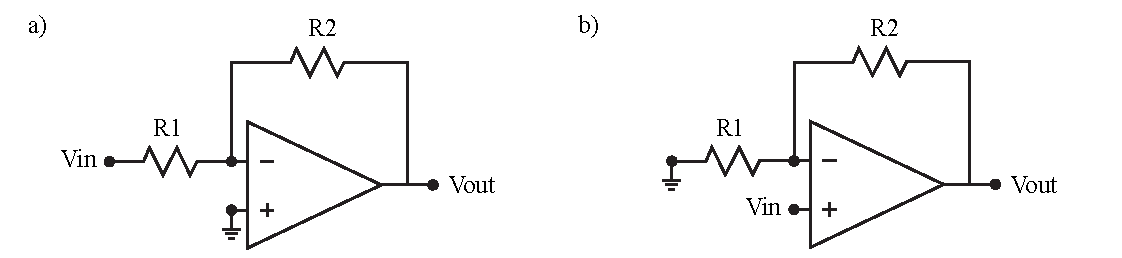
\includegraphics[width=1\textwidth]{Lab4configs.pdf}
	\caption{Different op amp configurations: inverting amplifier (a) and non-inverting amplifier (b)} \label{fig:OAconfigs}
\end{figure}

%%%%%%%%%%%%%%%%%%%%%%%%%%%%%%%%%%%%%%%%%%%%%%%%%%%%%%%%%%%%%%%%%%%%%%%%%%%%%%%%%%%%%%%%%%%%%%%%%%%%%%
\subsubsection{Inverting Amplifier}
%%%%%%%%%%%%%%%%%%%%%%%%%%%%%%%%%%%%%%%%%%%%%%%%%%%%%%%%%%%%%%%%%%%%%%%%%%%%%%%%%%%%%%%%%%%%%%%%%%%%%%

An inverting configuration, \hyperref[fig:OAconfigs]{Fiugre \ref*{fig:OAconfigs} (a)}, takes its name from the inversion that happens from input to output, giving a output voltage proportional to $R_2$ and $R_1$ independent of the actual op amp properties.

\begin{equation}
	\centering
	V_{out} =-\frac{R_2}{R_1}V_{in}
\end{equation}


%%%%%%%%%%%%%%%%%%%%%%%%%%%%%%%%%%%%%%%%%%%%%%%%%%%%%%%%%%%%%%%%%%%%%%%%%%%%%%%%%%%%%%%%%%%%%%%%%%%%%%
\subsubsection{Non-Inverting Amplifier}
%%%%%%%%%%%%%%%%%%%%%%%%%%%%%%%%%%%%%%%%%%%%%%%%%%%%%%%%%%%%%%%%%%%%%%%%%%%%%%%%%%%%%%%%%%%%%%%%%%%%%%

Similar to the inverting case, \hyperref[fig:OAconfigs]{Fiugre \ref*{fig:OAconfigs} (b)}, this configuration results in an output voltage proportional to R2 and R1 but without an inversion and always has a gain of at least 1.

\begin{equation}
	\centering
	V_{out} =(1+\frac{R_2}{R_1})V_{in}
\end{equation}

There is also a special case of the non-inverting amplifier where it is connected as a voltage follower or unity gain amplifier a show in \hyperref[fig:OAbuffer]{Figure \ref*{fig:OAbuffer}}.

\begin{figure} [h]
	\centering
		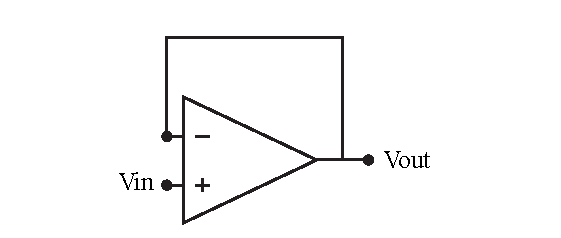
\includegraphics[width=0.5\textwidth]{Lab4buffer.pdf}
	\caption{A non-inverting amplifier configured as a unity gain buffer.} \label{fig:OAbuffer}
\end{figure}

The output is related directly to the input where

\begin{equation}
	\centering
	V_{out} = V_{in}
\end{equation}

\noindent and while this configuration may seem redundant, it has the advantage of providing a large input impedance to the source, $\mathrm{V_{in}}$, and a small output impedance to the load, $\mathrm{V_{out}}$. 

%%%%%%%%%%%%%%%%%%%%%%%%%%%%%%%%%%%%%%%%%%%%%%%%%%%%%%%%%%%%%%%%%%%%%%%%%%%%%%%%%%%%%%%%%%%%%%%%%%%%%%%
%\subsubsection{Summing Amplifier}
%%%%%%%%%%%%%%%%%%%%%%%%%%%%%%%%%%%%%%%%%%%%%%%%%%%%%%%%%%%%%%%%%%%%%%%%%%%%%%%%%%%%%%%%%%%%%%%%%%%%%%%
%
%A summing amplifier, \hyperref[fig:OAconfigs]{Fiugre \ref*{fig:OAconfigs} (c)}, is effectively the same configuration as an inverting amplifier but has multiple inputs that allow for a weighted output voltage. 
%
%\begin{equation}
	%\centering
	%V_{out} = -(\frac{R_4}{R_1}V_1 + \frac{R_4}{R_2}V_2 + \frac{R_4}{R_3}V_3)
%\end{equation}
%
%\noindent When the resistors $R_1$, $R_2$, $R_3$, and $R_4$ are all equal, the output voltage is an equal combination of the input voltages but the resistors can be chosen to weight the input voltages different based on the applicaiton. 
%
%
%%%%%%%%%%%%%%%%%%%%%%%%%%%%%%%%%%%%%%%%%%%%%%%%%%%%%%%%%%%%%%%%%%%%%%%%%%%%%%%%%%%%%%%%%%%%%%%%%%%%%%%
%\subsubsection{Difference Amplifier}
%%%%%%%%%%%%%%%%%%%%%%%%%%%%%%%%%%%%%%%%%%%%%%%%%%%%%%%%%%%%%%%%%%%%%%%%%%%%%%%%%%%%%%%%%%%%%%%%%%%%%%%
%
%Difference amplifiers, \hyperref[fig:OAconfigs]{Figure \ref*{fig:OAconfigs} (d)}, as the name implies takes the difference between the two input voltages resulting in that depends on the ratios of resistor values.
%
%\begin{equation}
	%\centering
	%V_{out} =  V_1 \left(\frac{R_2}{R_1+R_2}\right)\left(\frac{R_3+R_4}{R_3}\right)-V_2\frac{R_4}{R_3}  
%\end{equation}
%
%\noindent When the resistors $R_1 = R_3$ and $R_2 = R_4$ the output voltage simplifies to 
%
%\begin{equation}
	%\centering
	%V_{out} =  (V_1-V_2)\frac{R_2}{R_1}  
%\end{equation}

%%%%%%%%%%%%%%%%%%%%%%%%%%%%%%%%%%%%%%%%%%%%%%%%%%%%%%%%%%%%%%%%%%%%%%%%%%%%%%%%%%%%%%%%%%%%%%%%%%%%%%
\subsection{Op Amp Pins}
%%%%%%%%%%%%%%%%%%%%%%%%%%%%%%%%%%%%%%%%%%%%%%%%%%%%%%%%%%%%%%%%%%%%%%%%%%%%%%%%%%%%%%%%%%%%%%%%%%%%%%

A pinout is a connection diagram for an integrated circuit and shows which pins connect to which op amp terminals internally, not to be confused with the pins in a spice simulation. Op amps have a fairly common pinout resulting in chips that can be swapped out easily. \hyperref[fig:pinout]{Figure \ref*{fig:pinout}} shows the pinout for the TLV272 with the op amp diagram drawn within. 

\begin{figure} [h]
	\centering
		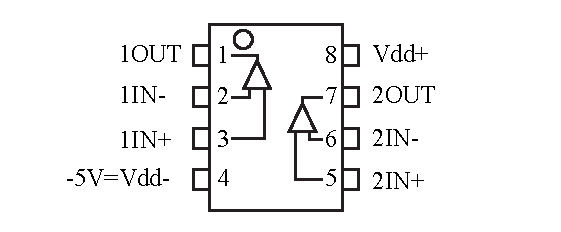
\includegraphics[width=0.5\textwidth]{Lab5pinout.pdf}
	\caption{Pinout for TI's TLV272. Note that two op amps are contained, often called a dual op amp, within a single chip.} \label{fig:pinout}
\end{figure}


\begin{table}[h]
\begin{center}
\begin{tabular}{|l|l|l|}
	\hline
	\textbf{Name} & \textbf{Number} & \textbf{Description} \\ \hline
	1OUT & 1 & Output of the first op amp \\ \hline
	1IN- & 2 & Inverting input of the first op amp \\ \hline
	1IN+ & 3 & Non-inverting input of the first op amp \\ \hline
	Vdd- & 4 & Negative supply, connected to ground for single supply operation \\ \hline
	2IN+ & 5 & Non-inverting input of the second op amp \\ \hline
	2IN- & 6 & Inverting input of the second op amp \\ \hline
	2OUT & 7 & Output of the second op amp \\ \hline
	Vdd+ & 8 & Positive supply \\ 
	\hline 
\end{tabular}
\end{center}
\caption{Pin descriptions from the TLV272 datasheet.}
\label{tbl:TLV272pinout}
\end{table}


The pins are numbered from 1 to 8 and count counter-clockwise starting in the upper left and the individual pin descriptions are in \hyperref[tbl:TLV272pinout]{Table \ref*{tbl:TLV272pinout}}. Most of the pins should be familiar from class.

Polarity or the orientation of the chip is determined by a circle or indentation on the chip itself, the TLV272 has a small circle indentation in the upper left hand corner to indicate polarity and the position of pin 1. 

%%%%%%%%%%%%%%%%%%%%%%%%%%%%%%%%%%%%%%%%%%%%%%%%%%%%%%%%%%%%%%%%%%%%%%%%%%%%%%%%%%%%%%%%%%%%%%%%%%%%%%%
%\subsection{Potentiometers}
%%%%%%%%%%%%%%%%%%%%%%%%%%%%%%%%%%%%%%%%%%%%%%%%%%%%%%%%%%%%%%%%%%%%%%%%%%%%%%%%%%%%%%%%%%%%%%%%%%%%%%%
%
%A potentiometer (or ``pot'') is a three terminal resistor as shown in \hyperref[fig:potcktdia]{Figure \ref*{fig:potcktdia}}. The resistance between terminals 1 and 3 is fixed and is equal to the rated value for the potentiometer. Terminal 2 is connected to a movable contact called the arm or wiper and the resistance between terminals 2 and 1 or between 2 and 3 can be varied by moving the arm. If terminals 1 and 3 are connected across a voltage source, then the voltage between terminals 2 and 1 or between 2 and 3 can be varied by moving the arm. In some cases, terminal 2 is connected to either terminal 1 or 3 so that the resistance from terminals 1 to 3 can be varied. 
%
%\begin{figure}[h] 
	%\centering
	%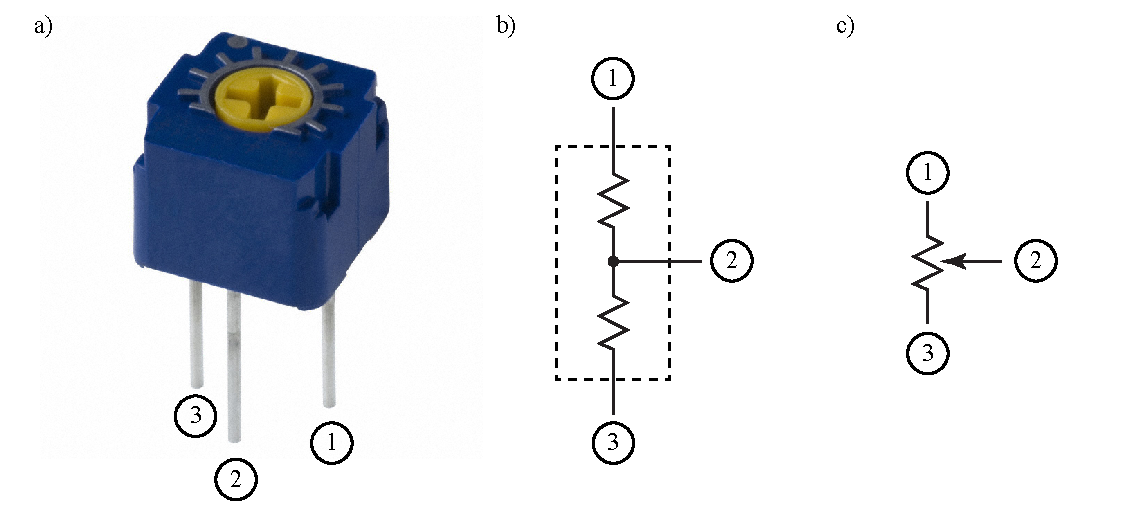
\includegraphics[width=1\textwidth]{lab2potdia.pdf}
	%\caption{A picture of a practical potentiometer with the appropriate pins labeled (a), an equivalent circuit diagram of a potentiometer with the wiper in a fixed position (b), and the common circuit schematic representation for a potentiometer (c).} \label{fig:potcktdia}
%\end{figure}

%%%%%%%%%%%%%%%%%%%%%%%%%%%%%%%%%%%%%%%%%%%%%%%%%%%%%%%%%%%%%%%%%%%%%%%%%%%%%%%%%%%%%%%%%%%%%%%%%%%%%%%
\section{Big Picture}
%%%%%%%%%%%%%%%%%%%%%%%%%%%%%%%%%%%%%%%%%%%%%%%%%%%%%%%%%%%%%%%%%%%%%%%%%%%%%%%%%%%%%%%%%%%%%%%%%%%%%%%

\begin{figure} [h]
	\centering
		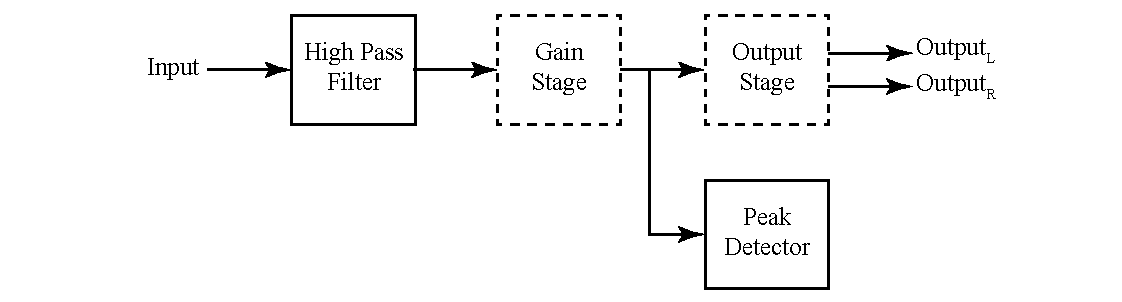
\includegraphics[width=1\textwidth]{Lab5bigpicture.pdf}
	\caption{Big picture with emphasis on the gain and output stages.} \label{fig:5bp}
\end{figure}

This lab focuses on op amps which will be used in the gain and outputs stages of the final project. 

%%%%%%%%%%%%%%%%%%%%%%%%%%%%%%%%%%%%%%%%%%%%%%%%%%%%%%%%%%%%%%%%%%%%%%%%%%%%%%%%%%%%%%%%%%%%%%%%%%%%%%%
\section{Pre-Lab Requirements}
%%%%%%%%%%%%%%%%%%%%%%%%%%%%%%%%%%%%%%%%%%%%%%%%%%%%%%%%%%%%%%%%%%%%%%%%%%%%%%%%%%%%%%%%%%%%%%%%%%%%%%%

Complete the following before coming to lab. 

%%%%%%%%%%%%%%%%%%%%%%%%%%%%%%%%%%%%%%%%%%%%%%%%%%%%%%%%%%%%%%%%%%%%%%%%%%%%%%%%%%%%%%%%%%%%%%%%%%%%%%%
\subsection{LTspice TLV272 Op Amp Model} \label{ssec:opampmodel}
%%%%%%%%%%%%%%%%%%%%%%%%%%%%%%%%%%%%%%%%%%%%%%%%%%%%%%%%%%%%%%%%%%%%%%%%%%%%%%%%%%%%%%%%%%%%%%%%%%%%%%%

Complete the following using the TLV271 spice model, always power the op amp with +/- 5 V for $V_{dd+}$ and $V_{dd-}$.

\begin{enumerate}
	\item Obtain the TLV2 spice model from TI's website: \url{http://www.ti.com/lit/zip/slom249}. Note that this is the model for the TLV271 which is the same op amp that's duplicated in the TLV272. If you have trouble accessing the zip file using the link, the file can also be accessed from the "lab related files" folder on canvas.
	\item Import the model in to LTspice using the instructions here: \url{http://www.linear.com/solutions/4678}. Make sure that the file, TLV271.lib, is extracted from the zip before opening and making the model, otherwise LTspice won't be able to reference the sub circuit file. Also, the pin numbers in the spice model correspond to the numbers in the sub circuit for the TLV272 and not the numbers in \hyperref[tbl:TLV272pinout]{Table \ref*{tbl:TLV272pinout}}.
	\item Read the TLV272 datasheet. \url{http://www.ti.com/lit/ds/symlink/tlv272.pdf}. Make sure note that pin 4 should be connected to -5 V, NOT ground. It is also recommended to use the schematic on page 42 rather than the schematic in the datasheet to avoid confusion when constructing your physical circuit.
	\item Using the voltage follower configuration in \hyperref[fig:OAbuffer]{Figure \ref*{fig:OAbuffer}}, run a DC operating point simulation (.op) and determine the $V_{out}$ when $V_{in}$ is zero volts; effectively calculating the offset voltage, table the value. 
	\item With the same voltage follower configuration, \hyperref[fig:OAbuffer]{Figure \ref*{fig:OAbuffer}}, set $V_{in}$ to a 1 V amplitude pulse. Vinitial(V): 0, Von(V): 1, Tdelay(s): 0.5m, Ton(s): 10s, Ncycle: 100. Leave any remaining variables blank. Run a transient analysis with a stop time of 1m (.tran 1m). Plot the input and output voltage from 495 us to 505 us and then find then the time it takes for the output to reach 1 V, the time should be on the order of micro seconds. This is a measure of slew rate in V/us, table the value. Save an image of the circuit and the plot of the input and output voltage for submission to canvas. \label{itm:5ssec1itm5}
	\item Configure an inverting amplifier, \hyperref[fig:OAconfigs]{Fiugre \ref*{fig:OAconfigs} (a)}, with a gain of 10 by setting $R_2=10\mathrm{k}$ and $R_1 = 1 \mathrm{k}$. Set the input voltage to a sine wave with the following parameters, DC offset(V): 0, Amp(V): 1, Freq(Hz): 1k, and the remaining variables blank. Run a transient analysis with a stop time of 1m (.tran 1m). Plot the input and output voltage and record the max and min values of $V_{out}$, this is a measure of the maximum output swing, table the value. Save an image of the circuit and the plot of the input and output voltage for submission to canvas. \label{itm:5ssec1itm6}
	\item Using the same inverting configuration, \hyperref[fig:OAconfigs]{Fiugre \ref*{fig:OAconfigs} (a)},set $V_{in}$ to a 0.1 V DC source and run a transient analysis with a stop time of 1m (.tran 1m). Plot $-V(vout)/V(vin)$, this is a measure of the effective gain, table the result. Save an image of the circuit and the plot of effective gain for submission to canvas. \label{itm:5ssec1itm7}
\end{enumerate}

%%%%%%%%%%%%%%%%%%%%%%%%%%%%%%%%%%%%%%%%%%%%%%%%%%%%%%%%%%%%%%%%%%%%%%%%%%%%%%%%%%%%%%%%%%%%%%%%%%%%%%%
\subsection{Op Amp Construction} \label{ssec:opampcon}
%%%%%%%%%%%%%%%%%%%%%%%%%%%%%%%%%%%%%%%%%%%%%%%%%%%%%%%%%%%%%%%%%%%%%%%%%%%%%%%%%%%%%%%%%%%%%%%%%%%%%%%

\begin{figure} [h]
	\centering
		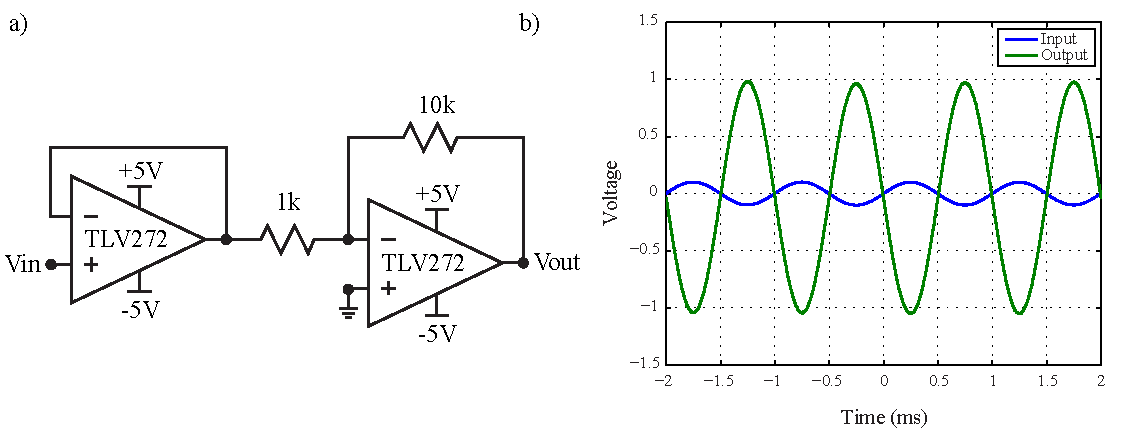
\includegraphics[width=1\textwidth]{Lab5demockt.pdf}
	\caption{Schematic for the demo circuit, a voltage follower followed by an inverting amplifier with a gain of 10 (a) and the resulting output (b)} \label{fig:5demockt}
\end{figure}

\begin{enumerate}
	\item Using only one of the TLV272 op amp in your lab parts kit, build the circuit in \hyperref[fig:5demockt]{Figure \ref*{fig:5demockt} (a)} on a breadboard. Set the voltage supplies to +/- 5 V and scope channel 1 to Vin and scope channel 2 to Vout. Configure the Wavegen to supply a 1 kHz sine wave with a 0.1 V amplitude. 
\end{enumerate}

%%%%%%%%%%%%%%%%%%%%%%%%%%%%%%%%%%%%%%%%%%%%%%%%%%%%%%%%%%%%%%%%%%%%%%%%%%%%%%%%%%%%%%%%%%%%%%%%%%%%%%%
\section{In-Lab Requirements}
%%%%%%%%%%%%%%%%%%%%%%%%%%%%%%%%%%%%%%%%%%%%%%%%%%%%%%%%%%%%%%%%%%%%%%%%%%%%%%%%%%%%%%%%%%%%%%%%%%%%%%%

The following must be completed at the start of lab. 

\begin{enumerate}
	\item All of the theoretical parameters from \hyperref[ssec:opampmodel]{Subsection \ref*{ssec:opampmodel}} tabled:
		\begin{enumerate}
			\item Offset voltage.
			\item Slew rate.
			\item Maximum output swing. 
			\item Effective gain. 
		\end{enumerate}
	\item Images of the output and circuits from \hyperref[ssec:opampmodel]{Subsection \ref*{ssec:opampmodel}} tabled:
		\begin{enumerate}
			\item \hyperref[itm:5ssec1itm5]{Item \ref*{itm:5ssec1itm5}}: Image of the circuit and the plot of the input and output voltage.
			\item \hyperref[itm:5ssec1itm6]{Item \ref*{itm:5ssec1itm6}}: Image of the circuit and the plot of the input and output voltage.
			\item \hyperref[itm:5ssec1itm7]{Item \ref*{itm:5ssec1itm7}}: Image of the circuit and the plot of effective gain.
		\end{enumerate}
	\item Op amp configurations from \hyperref[ssec:opampcon]{Subsection \ref*{ssec:opampcon}} built on a breadboard and working.
\end{enumerate}

%%%%%%%%%%%%%%%%%%%%%%%%%%%%%%%%%%%%%%%%%%%%%%%%%%%%%%%%%%%%%%%%%%%%%%%%%%%%%%%%%%%%%%%%%%%%%%%%%%%%%%%
\subsection{Experimental Op Amp Measurements}
%%%%%%%%%%%%%%%%%%%%%%%%%%%%%%%%%%%%%%%%%%%%%%%%%%%%%%%%%%%%%%%%%%%%%%%%%%%%%%%%%%%%%%%%%%%%%%%%%%%%%%%

Using the pre-built op amp configurations, complete the following.

\begin{enumerate}
	\item Using the voltage follower, \hyperref[fig:OAbuffer]{Figure \ref*{fig:OAbuffer}},input a 0 V DC voltage from the Wavgen and record the offset voltage. Choose an appropriate voltage scale, the voltage is on the order of mV. Save a screenshot of the waveform scope.
	\item Using the voltage follower again, \hyperref[fig:OAbuffer]{Figure \ref*{fig:OAbuffer}}, input a 0.5 V amplitude square wave with a 0.5 V offset from the Wavegen. Set the appropriate trigger and determine the slew rate in V/us. Save a screenshot of the waveform scope.
	\item Using the inverting amplifier, \hyperref[fig:OAconfigs]{Fiugre \ref*{fig:OAconfigs} (a)}, input a 1k Hz sine wave with a 1 V amplitude from the Wavegen. Determine the maximum output voltage swing. 
	\item Using the inverting amplifier again, \hyperref[fig:OAconfigs]{Fiugre \ref*{fig:OAconfigs} (a)}, input a 0.1 V DC from the Wavegen. Determine the effective gain. Choose an appropriate voltage scale for the input and output voltages. 
	\item Table all of values calculated in this subsection.
\end{enumerate}


%%%%%%%%%%%%%%%%%%%%%%%%%%%%%%%%%%%%%%%%%%%%%%%%%%%%%%%%%%%%%%%%%%%%%%%%%%%%%%%%%%%%%%%%%%%%%%%%%%%%%%%
\section{Write Up}
%%%%%%%%%%%%%%%%%%%%%%%%%%%%%%%%%%%%%%%%%%%%%%%%%%%%%%%%%%%%%%%%%%%%%%%%%%%%%%%%%%%%%%%%%%%%%%%%%%%%%%%

Include the following in the write up.

\begin{enumerate}
	\item Table of experimental parameters.
	\item Screenshots of scope output plots.
	\item Percent error, using the pre-lab values as the theoretical and the in-lab values as experimental.
\end{enumerate}

Discuss the differences between the ideal op amp model, spice TLV272 model, and the physical op amp focusing on the quantities calculated for this lab: offset voltage, slew rate, output voltage range, and effective gain. Touch on the following in your discussion.

\begin{itemize}
	\item When is it appropriate to use one model over the other?
	\item How accurate should the spice model for an op amp be?
\end{itemize}
For all lab write up submissions and reports the backgrounds for LTSpice and Waveforms should be changed from dark background to light background to make them readable for grading. 

If the prelab simulation is incorrect, do not compare the in lab results to wrong values.  Correct numbers or circuit schematics should be used in the write-up report.
